\documentclass[Arkitektur/System_main.tex]{subfiles}
\begin{document}
\section{Deployment View}
I dette afsnit beskrives det fysiske standpunkt af systemet. Her beskrives toplogien af software komponenter på det fysiske lag såvel som de fysiske forbindelser mellem disse komponenter. For at illustrere dette, er det lavet et deployment diagram.
I diagrammet vises de tre lag applikationen opererer i, og hvordan hardware og softwarekomponenterne interagerer med hinanden: visualiseringen af hardwareprocessorne og placering af softwareelementer på pågældende hardware. 

Lagene kan opdeles i tre 'tiers': Presentation, Business og Data.\\
\begin{figure}[H]
    \centering
    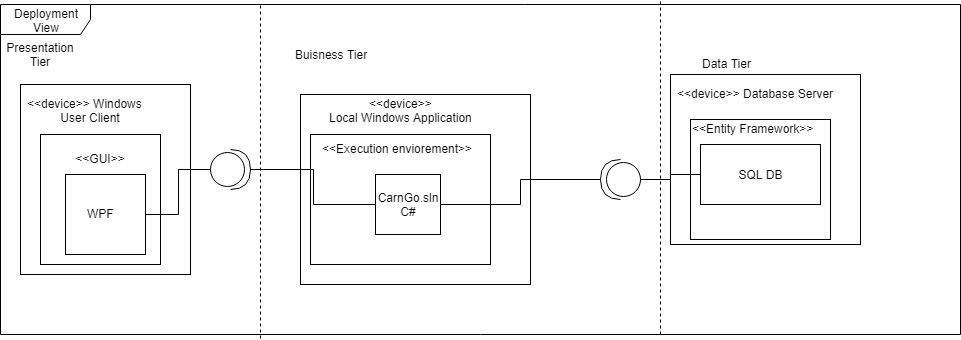
\includegraphics[width=\linewidth]{Arkitektur/4+1View/Graphics/DeploymentDiagram.png}
    \caption{Deployment View}
\end{figure}
'Presentation tier' fremviser de dele af systemet, som brugeren interagerer med. Den første del er 'Windows User Client', som repræsenterer selve applikationen, som brugeren benytter - brugeren interagere via skærm, keyboard og mus (Grafisk brugeroverflade). Denne brugeroverflade visualiseres ved brug af frameworket WPF, den specifikke struktur er MVVM. Heri indgår også ViewModellerne, som angiver præsentationslogikken (Hvile data skal vises på den grafiske brugeroverflade). Presentatationsniveauet er forbundet til forretningslogikken. 'Business Tier' behandler den information og inputs, som sendes fra Client. "Execution enviroment' angiver eksekveres miljøet, som behandler alt informationen og udfører de logiske operationer omhandlende forretningslogikken - det kunne fx være validering eller kommunikation til databasen. Softwaren er skrevet i C\#.  

Business Tier er forbundet til et Data Tier, som er den del af applikationen, der indeholder en database. Databasen gemmer informationer omkring brugeren og deres interaktioner i form af et beskedsystem. Til at opbevarer denne information anvendes Microsoft Azure, som er en cloudcomputing platform, der gør det muligt at lagre data. Databasen bliver realiseret gennem Entity Framework Core, hvor SQL bruges til implementeringen af opbevaringsstrukturen. EF Core gør det også muligt at skabe et bindeled mellem Business Tier og Data Tier. 
\end{document}